\documentclass[a4paper,12pt]{article}
\usepackage{amssymb} % needed for math
\usepackage{amsmath} % needed for math
\usepackage[default]{helvet}
\usepackage[utf8]{inputenc} % this is needed for german umlauts
\usepackage[ngerman]{babel} % this is needed for german umlauts
\usepackage[T1]{fontenc}    % this is needed for correct output of umlauts in pdf
\usepackage[margin=2.5cm]{geometry} %layout
\usepackage{booktabs}
\usepackage{xcolor}

% this is needed for forms and links within the text
\usepackage[hidelinks]{hyperref}  

\usepackage{pdflscape} % für Seiten im Querformat

\setlength{\parindent}{0em} % verhindert den Einzug neuer Zeilen nach einem "\par"

% Bold figure captions
\usepackage{caption}
\captionsetup[figure]{labelfont=bf}

\usepackage{multicol} % Erlaubt es mit dem Zusatz \begin{multicols}{x} zu bestimmen, dass "x" Spalten angelegt werden sollen. So kann man Items auf mehrere Spalten verteilen.

% float-enviroments for figures and tables
\usepackage{float}

% The following is needed in order to make the code compatible
% with both latex/dvips and pdflatex.
\ifx\pdftexversion\undefined
\usepackage[dvips]{graphicx}https://www.overleaf.com/project/653ecd36a364a3e0e12e8cbd
\else
\usepackage[pdftex]{graphicx}
\DeclareGraphicsRule{*}{mps}{*}{}
\fi

% legt Standardpfad für Abbildungen fest
\graphicspath{ {./Abbildungen/} }

%%%%%%%%%%%%%%%%%%%%%%%%%%%%%%%%%%%%%%%%%%%%%%%%%%%%%%%%%%%%%%%%%%%%%%
% Variablen                                 						 %
%%%%%%%%%%%%%%%%%%%%%%%%%%%%%%%%%%%%%%%%%%%%%%%%%%%%%%%%%%%%%%%%%%%%%%
\newcommand{\authors}{Martin Kriger, Maximilian Reiner, Michael Brüggemann, Tim Ciroth, Leonard Wittrock}
\newcommand{\auftraggeber}{Institut für Geoinformatik, Universität Münster}
\newcommand{\auftragnehmer}{M3TL}
\newcommand{\projektName}{Web based Machine Learning for OpenEOcubes - WebMLOpenEO}
\newcommand{\tags}{\authors, Pflichtenheft, ML, Remote Sensing}
\newcommand{\glossarName}{Glossar}

%%%%%%%%%%%%%%%%%%%%%%%%%%%%%%%%%%%%%%%%%%%%%%%%%%%%%%%%%%%%%%%%%%%%%%
% Informations for the title page                                 						 %
%%%%%%%%%%%%%%%%%%%%%%%%%%%%%%%%%%%%%%%%%%%%%%%%%%%%%%%%%%%%%%%%%%%%%%

\title{\projektName~(Pflichtenheft)}
\author{Martin Kriger, Michael Brüggemann, Tim Ciroth, Leonard Wittrock}
\date{\today}

%%%%%%%%%%%%%%%%%%%%%%%%%%%%%%%%%%%%%%%%%%%%%%%%%%%%%%%%%%%%%%%%%%%%%%
% PDF Meta information                                 				 %
%%%%%%%%%%%%%%%%%%%%%%%%%%%%%%%%%%%%%%%%%%%%%%%%%%%%%%%%%%%%%%%%%%%%%%
\hypersetup{
  pdfauthor   = {\authors},
  pdfkeywords = {\tags},
  pdftitle    = {\projektName~(Pflichtenheft)}
} 

    
 
%%%%%%%%%%%%%%%%%%%%%%%%%%%%%%%%%%%%%%%%%%%%%%%%%%%%%%%%%%%%%%%%%%%%%%
% Create a shorter version for tables. DO NOT CHANGE               	 %
%%%%%%%%%%%%%%%%%%%%%%%%%%%%%%%%%%%%%%%%%%%%%%%%%%%%%%%%%%%%%%%%%%%%%%
% nimmt 3 Parameter entgegen, die an den Stellen #1, #2, #3 ausgegeben werden. Die "&" werden gebraucht, da die rows in einem "tabular" enviroment verwendet werden
\newcommand{\addrow}[3]{#1 &#2 &#3 \\ [0.2cm]}


\newcommand{\addheading}[3]{#1 &#2 &#3\\ \hline }
\newcommand{\tabularhead}{\begin{tabular}{l p{5cm} p{8cm}}
\hline
}

\newcommand\addmulrow[2]{ \begin{minipage}[t][][t]{2.5cm}#1\end{minipage}% 
   &\begin{minipage}[t][][t]{8cm}
    \begin{enumerate} #2   \end{enumerate}
    \end{minipage}\\ }


\newenvironment{usecase}{\tabularhead}
{\hline\end{tabular}}


%%%%%%%%%%%%%%%%%%%%%%%%%%%%%%%%%%%%%%%%%%%%%%%%%%%%%%%%%%%%%%%%%%%%%%
% Wie nutze ich einen Usecase??          	                         %
%%%%%%%%%%%%%%%%%%%%%%%%%%%%%%%%%%%%%%%%%%%%%%%%%%%%%%%%%%%%%%%%%%%%%%
% 1. Envirment mit \begin{usecase} öffnern
% 2. mit \addheadheading{}{}{} drei Tabellenüberschriften vergeben
% wenn die Spalte "Bezug" (zweite Spalte) zu voll ist, kann es sein, dass der vertikale Abstand zwischen 2 Zeilen nicht ordentlich dargestellt wird


%%%%%%%%%%%%%%%%%%%%%%%%%%%%%%%%%%%%%%%%%%%%%%%%%%%%%%%%%%%%%%%%%%%%%%
% THE DOCUMENT BEGINS             	                              	 %
%%%%%%%%%%%%%%%%%%%%%%%%%%%%%%%%%%%%%%%%%%%%%%%%%%%%%%%%%%%%%%%%%%%%%%
\begin{document}
 \pagenumbering{roman}
 
\begin{titlepage}

	\begin{figure}[!tbp]
	  \centering
	  \begin{minipage}[b]{0.3\textwidth}
		
\includegraphics[width=\textwidth]{Logo_UniMuenster_.jpg}
	  \end{minipage}
	  \hfill
	  \begin{minipage}[b]{0.3\textwidth}
		
\includegraphics[width=\textwidth]{M3TL_Logo.jpeg}
	  \end{minipage}
	\end{figure}
	
	
	\maketitle
	\thispagestyle{empty} % no page number
	
	
	% fill space till next text
	\vspace*{\fill}
	
	  \begin{tabular}[t]{ll}
		Projekt:       & \quad \projektName \\[1.2ex]
		Auftraggeber:  & \quad \auftraggeber\\[1.2ex]
		Auftragnehmer: & \quad \auftragnehmer\\[1.2ex]
	  \end{tabular}
	
	\newpage
	
	\begin{tabular}{|p{3 cm}|p{3 cm}|p{7 cm}|}
	\hline
	\textbf{Version} & \textbf{Datum} & \textbf{Autor(en)} \\
	\hline
	\hline
	1.0 & 06.11.2023 & \authors \\
	\hline
	1.1 & 10.12.2023 & \authors \\
	\hline
	\end{tabular}
	
	% die Versionsseite könnte man auch noch weiter verschieben
	\end{titlepage}
	
         % Deckblatt.tex laden und einfügen
 \setcounter{page}{3}
 \tableofcontents          % Inhaltsverzeichnis ausgeben
 \clearpage
 \pagenumbering{arabic}

\section{Zielbestimmung} \label{zielbestimmung}
Das Hauptziel dieses Projektes besteht darin, einen openEO-Dienst zu entwickeln und zu implementieren, der die Klassifizierung von Fernerkundungsbildern auf Grundlage eines Trainingsdatensatzes mit dem Random-Forest Algorithmus ermöglicht. Hierbei sollen bestehende Lösungen wie openEO-Cubes verwendet und um neue Funktionen erweitert werden. Ein essenzieller Bestandteil des Projekts ist die Integration eines innovativen Prozesses in die vorhandenen openEO-Abläufe. Der von uns entwickelte Prozess erwartet einen Trainingsdatensatz, der Informationen zu bekannten Klassen und ihren Standorten enthält, die Spezifikation von Hyperparametern sowie einer Area of Interest (AOI), welche zu klassifizieren sein soll. Die Ergebnisse der Klassifizierung sollen daraufhin auf zwei Arten zugänglich gemacht werden. Als eine interaktive Visualisierung mittels einer webbasierten Browseranwendung und als Downloadmöglichkeit.
\par
Das Projekt strebt an, eine benutzerfreundliche und leistungsstarke Plattform zu schaffen, die nicht nur die Klassifizierung von Fernerkundungsbildern ermöglicht, sondern auch eine intuitive Interaktion und den Zugang zu den Ergebnissen sowohl für die Forschungsgemeinschaft als auch für interessierte Nutzerinnen und Nutzer erleichtert.

\section{Produkteinsatz} \label{produkteinsatz}
Die Zielnutzer sind Forscher oder Fachleute im Bereich Fernerkundung und räumliches Modellieren, die maschinelles Lernen für LULC-Klassifikationen nutzen möchten. Sie verlassen sich auf Sentinel-2-Satellitenbilder für ihre Projekte, beherrschen das Training und die Anwendung von Machine-Learning-Modellen und sind an groß angelegten Kartierungs- bzw. Modellierungsanwendungen interessiert, verfügen jedoch nicht über die Hardwarekomponenten, um maschinelles Lernen auf großen Datensätzen durchzuführen. Das Produkt soll auf den eigenen Servern zu betreiben sein, um technologische Barrieren für Benutzer zu minimieren, die ihre Modelle in alltäglichen Bildanalyseaufgaben ausführen und bewerten möchten. Dieser Dienst soll leicht anwendbar und flexibel sein und gewährleistet eine einfache Infrastruktur für ähnliche Anwendungsfälle.


\section{Produktbeschreibung} \label{produktbeschreibung}
\par
Unser Produkt stellt einen umfassenden Webservice zur Verfügung, welcher aus einem Frontend-Server, einem Node.js-Backend und einem OpenEO-konformen R Backend besteht.
Der Frontend Server stellt der Nutzer:in eine gerenderte HTML Seite zur Verfügung, auf der die Klassifikationsaufgabe konfiguriert werden kann. Der Frontendserver stellt ebenfalls eine HTML mit der Dokumentation zu unserem Webservice zur Verfügung.  Durch das Verwenden von Vue.js ist außerdem eine umfangreiche Browserunterstützung gewährleistet (90\%).
\par
Im Node.js-Backend werden die Anfragen des Users gebündelt. Dort wird eine API bereitgestellt, die die Services unserer Anwendung beschreibt (API-self-documentation), sowie die Anfragen der Nutzer:innen verarbeitet, bzw. in neue Anfragen an andere Server umwandelt (Routing).
\par
Die Anfragen zu einer Klassifikation werden dann an ein OpenEO-konformes Backend weitergeleitet, auf welchem die tatsächlichen Berechnungen stattfinden. Dieses nutzt die bereits bestehenden Strukturen von 'openEOcubes' und erweitert diese um geeignete Prozesse, um die machine-learning gestützte Klassifikation durchzuführen. So werden bereits bestehende Prozesse zur Verbarbeitung von Datacubes durch 'openEOcubes' genutzt und auch neue Prozesse im Bereich machine-learning ergänzt.
\par
Der Webservice selbst wird auf DockerHub als Docker-Image bereitgestellt, welches direkt auf einer Amazon AWS/EC2 Instanz gehostet wird. So ist sichergestellt, dass der Service unabhängig vom lokalen System ausgeführt wird und der Webservice dadurch ebenfalls über die für die Klassifikationen nötige Rechenleistung verfügt.
Dieses Docker Image besteht dabei aus 3 Services. Dies sind die oben beschriebenen Komponenten des Services (Frontend, Node.js-Backend, R Backend). Da jede Komponente nur eine einzelne Programmiersprache nutzt, kann auf komplexe Build-Prozesse mit Makefiles verzichtet werden. Unser Entwicklungsprozess besteht hier aus in den Testsuites 'Jest', 'vitest' und 'testthat' definierten Unit- und Integrations-Tests, sowie einem nach dem 4-Augenprinzip überwachten Pullrequest-Prozess in unserem Github-Repository.
\par
% ggf. müssen wir hier genau definieren, welche Lizenz wir nutzen
Der gesamte Webservice wird unter einer OSI Lizenz veröffentlicht und steht als OpenSource-Software zur Verfügung. Der Kunde erhält über unser GitHub Repository während des Entwicklungsprozesses Zugriff auf den Quellcode, sowie alle dort verwalteten Projektmanagementdokumente (siehe Abschnitt \ref{zugang}).


\section{Funktionale Anforderungen}
%%%%%%%%%%%%%%%%%%%%%%%%%%%%%%%%%%%%%%%%%%%%%%%%%%%%%%%%%%%%%%%%%%%%%%
% Was muss das Programm können?                   					 %
%%%%%%%%%%%%%%%%%%%%%%%%%%%%%%%%%%%%%%%%%%%%%%%%%%%%%%%%%%%%%%%%%%%%%%

\subsection{Data Ingest}

\begin{usecase}

    %Data Ingest Funktionale Anforderungen
  \addheading{Nummer}{Bezug}{Beschreibung} 
  \addrow{/FA05/}{}{Unsere Web-App wird als eine One-Page-Struktur implementiert, welche auf der Hauptseite ein Formular besitzt, um die benötigten Daten für die Verarbeitung einzugeben und einzuladen.} 
  \addrow{/FA10/}{support loading training data via direct file upload to the server, support at least file formats GeoJSON and GeoPackage}{Im Formular wird ein Button bereitgestellt, der den File-Explorer öffnet, um Dateien für die Trainingsdaten hochzuladen. GeoJSON und GeoPackage werden unterstützt.} 
  \addrow{/FA15/}{the server automatically discovers and processes (accesses, or downloads) the
satellite imagery from other sources as required for model training and prediction based on the locations and extents of the area of interest and training
data} {Mithilfe einer STAC API werden die Satellitenbilder, welche auf einem S3 Bucket bei AWS liegen angefragt, sodass entwickelte Prozessgraphen mit übergebenen Argumenten zur AOI und dem Trainingsgebiet weitere Argumente nutzen können. Hierfür verwenden wir die R Bibliothek 'rstac'.}
  \addrow{/FA20/}{the server automatically discovers and processes (accesses, or downloads) the
satellite imagery from other sources as required for model training and prediction based on the locations and extents of the area of interest and training
data, /F05/}{Durch die gleichzeitige und gemeinsame Speicherung auf einer AWS-Instanz (us-west-2 region Oregon) wird der direkte Zugriff auf die Collection der Erdbeobachtungsdaten des Sentinel-2 Satelliten möglich.}
  \addrow{/FA25/}{example satellite data for demonstration purposes is being kept available on the
server}{Unsere Anwendung bietet die Möglichkeit über einen Button einen Demoprozess zu starten. Dies ist ein geführter Prozess, indem die Nutzer:in eine mögliche Eingabe in unseren Webservice vorgestellt bekommt und diese Anfrage dann an den Server gesandt wird.}

\end{usecase}

\subsection{Processes}

\begin{usecase}
  %Processes Funktionale Anforderungen
  \addheading{Nummer}{Bezug}{Beschreibung} 
  \addrow{/FA30/}{implement at least one standard machine learning algorithm for LULC classification supporting training and prediction on data cubes holding Sentinel-2 satellite image data}{Wir implementieren den 'Random Forest' Algorithmus. Random Forest zeichnet sich durch eine Hohe Performanz in LULC Klassifikationsproblemen aus und ist daher gut für diese Anwendung geeginet}
  \addrow{/FA35/}{allow the user to specify the target area by means of polygon data (e.g.by file upload, or on-screen digitizing).}{Der Nutzer wird die Möglichkeit haben in einer Karte, welche auf openLayers basiert, mithilfe eines Zeichenwerkzeuges, einen Kartenausschnitt mit der Area of Interest (AOI) einzuzeichnen.}
  \addrow{/FA40/}{allow the user to specify the target area by means of polygon
data (e.g. by file upload, or on-screen digitizing)
}{Optional kann eine GeoJSON-Datei, welche den gewünschten Bereich als beliebiges Polygon definiert, über einen Button, welcher den File-Explorer öffnet, hochgeladen werden.}
  \addrow{/FA45/}{allow the user to specify the target area (rectangular) and date
}{Neben der Möglichkeit einen Kartenausschnitt zu bestimmen, ist es möglich im Formular über eine Datumsauswahl, den Zeitpunkt für die gewünschten Satellitendaten, festzulegen.}
  \addrow{/FA55/}{allow the user to specify a lower resolution to compute predic-
tions on than the native resolution of the satellite imagery used}{Wir stellen ein Input Feld zur Verfügung, in der die Resolution des Satellitenbildes eingestellt werden kann. Im Backend wird dies durch 'openEOcubes' in Verbindung mit 'gdalcubes' realisiert.}
  \addrow{/FA60/}{in addition to the classified map, create and return the map with class probabilities of all classes of that for which the probability is maximum.}{Nach der Prozessierung wird dem Nutzer, über die Interaktive Karte, eine Möglichkeit gegeben die verschiedenen Kartentypen (predicted map, map with class probabilities) als Layerwechsel anzeigen zu lassen.}
  \addrow{/FA65/}{improve openEOcubes and submit one or more pull requests to its GitHub repo}{Die Erweiterung wird ein neu definierter openEO-Prozess sein, der das Berechnen einer LULC-Klassifikation mit dem Algorithmus 'Random Forest' ermöglicht und dabei auf dem Backend laufen wird. Zusätzlich dazu werden die Teilprozesse einer ML-Klassifikation als openEO-konforme Prozesse implementiert.}

\end{usecase}

\subsection{Visualisation}



\begin{usecase}
  %Visualisation Funktionale Anforderungen
  \addheading{Nummer}{Bezug}{Beschreibung} 
  \addrow{/FA70/}{visualize the training areas/locations (if applicable) and area of interest on an interactive map (leaflet, openlayers or similar)}{Die Web-App verfügt über eine Kartenansicht, die je nach ausgewähltem Schritt entweder die 'Area of Interest' oder die Training-Areas anzeigt.}
  \addrow{/FA75/}{visualize the resulting prediction (classification) on an interactive web map}{Nach Abschluss des Prozesses zeigt die Karte das Ergebnis in Form eines ein- und ausblendbaren Klassifizierungs-Layers an. Dieser Layer verwendet eine barrierefreie Farblegende, die auf Grundlage der vom Backend gelieferten Daten berechnet wird. Die Farblegende ermöglicht den Benutzern eine klare und zugängliche Darstellung der Klassifizierungsinformationen auf der Karte, wodurch sie die Ergebnisse leicht verstehen können.}
  \addrow{/FA80/}{visualize the resulting quality of prediction (e.g. probibility of
the most likely class) on an interactive web map}{Am Ende des Prozesses hat der Nutzer die Möglichkeit, eine Karte mit den Klassenwahrscheinlichkeiten in der Web-App anzuzeigen.}

\end{usecase}

\subsection{Data Download}

\begin{usecase}
  %Data Download Funktionale Anforderungen
  \addheading{Nummer}{Bezug}{Beschreibung} 
  \addrow{/FA85/}{enable the download of the prediction map in a standard raster data format}{  Unsere Web-App bietet einen Download-Button an, der es den Benutzern ermöglicht, die Rasterdaten im .TIFF-Format herunterzuladen.}
  \addrow{/FA90/}{enable download of the trained model (if applicable)}{Es wird eine Möglichkeit geben, das trainierte Model im '.rds' Format herunterzuladen.}

\end{usecase}

\subsection{Deployment}

\begin{usecase}

  %Deployment Funktionale Anforderungen  
  \addheading{Nummer}{Bezug}{Beschreibung} 
  \addrow{/FA95/}{Docker/docker-compose configurations are used for packaging and deployment}{Das Projekt besteht aus drei Docker-Services: ein HTTP-Server mit Vue.js, ein Node.js-Server und ein R-Server mit openEOcubes. Diese Services sind für die Bereitstellung der Benutzeroberfläche und  serverseitige Logik verantwortlich.}
  \addrow{/FA100/}{the developed system can be deployed to any host system without additional
software requirements other than recent versions of Docker/docker-compose}{Das Projekt kann mit Docker Compose gestartet werden, was die einfache Verwaltung und Bereitstellung der Anwendung ermöglicht.}
\textcolor{red}{}
\addrow{\textcolor{red}{/FA105/}}{\textcolor{red}{eigene Implementierung}}{\textcolor{red}{Alle Endpunkte unserer API im Node-Backend werden OpenAPI konform implementiert sein. Dies hat den Vorteil, dass unser Service nicht nur über die Website (als GUI) bedienbar ist,
sondern auch direkt aus anderen Clients (Python, R, JS) per HTTP-Requests genutzt werden kann.}}
\addrow{\textcolor{red}{/FA110/}}{\textcolor{red}{eigene Implementierung}}{\textcolor{red}{Wir integrieren eine technische Umsetzung einer Swagger API-Dokumentation für unser Projekt.
Obwohl dies nicht explizit in den anfänglichen Anforderungen aufgeführt war,
soll diese Dokumentation die technische Umsetzung unserer Endpunkte zeigen und detaillierte Einblicke in die zugrundeliegende Implementierung bieten.}}


\end{usecase}

\section{Nichtfunktionale Anforderungen}
Die meisten nichtfunktionalen Anforderungen werden bereits in dem Abschnitt 'Produkt-Umgebung' dargestellt (siehe Abschnitt \ref{produktbeschreibung}). Folglich wird hier weiterführend auf die Performance eingegangen.
\subsection{Performance}
Eine Änderung auf der Website erfolgt innerhalb einer Sekunde. Alle Inhalte werden asynchron geladen. Die interaktive Bedienung erfolgt innerhalb 0.1 Sekunden.


\section{Architektur}


\subsection{Systemarchitektur} \label{chpt:systemarchitecture}
Unsere Applikation nutzt eine Kombination aus einem Frontend-Server, sowie zwei Backend-Servern (Node-Backend und R-Backend) (vgl. Abb. \ref{fig:systemarchitecture}, im Anhang).

\subsubsection{Frontend-Server}
Der Frontend-Server stellt die HTML Seiten für die Nutzer:innen zur Verfügung, sowie einem Formular um mit der API unserer Applikation zu interargieren. Dort kann die Nutzer:in folgende Angaben machen:
\begin{multicols}{2}
\begin{enumerate}
    \item 'machine-learning' (ML) Model
    \item 'Area of Interest' 
    \item 'Time of Interest' (TOI)
    \item Trainingsdaten
    \item Hyperparameter
    \item Auflösung der Satellitenbilder
\end{enumerate}
\end{multicols}

Die Angabe des Models wählt aus, welches ML Model zur Klassifikation genutzt werden soll.
\par

Die AOI sowie die Trainingsdaten kann die Nutzer:in über eine interaktive Karte angeben. Trainingsdaten können alternativ als GeoJSON oder Geopackage direkt hochgeladen werden. Die dort erzeugten Geometrien werden dann zu einer GeoJSON codiert und mit dem Formular übergeben. 
\par
Die TOI bestimmt ein Zeitintervall, in welchem die Sentinel-2 Satellitendaten herangezogen werden sollen.
\par
Werden Hyperparameter für das Modell angegeben, so werden diese direkt für das zu trainierende ML Model verwendet. Da diese Parameter ggf. nicht optimal sein könnten, wird der Nutzer:in eine entsprechende Warnung gegeben. Werden keine Hyperparameter übergeben, so werden im R-Backend entsprechende Tuning-Methoden angewandt, um die optimalen Parameter zu ermitteln.
\par
Mit der Auflösung kann bestimmt werden, wie groß ein Pixel des Satellitenbildes sein soll. Je feiner die gewählte Auflösung, desto präzisere Klassifikation sind möglich, aber auch der Klassifikationsaufwand ist deutlich erhöht.

\subsubsection{Node-Backend}
Das Node-Backend stellt die API zur Verfügung und verwaltet Anfragen an diese (über den Browser einer Nutzer:in oder einen HTTP-Request aus einem Client (R, JS, Python, etc.)). Dort werden die Requests validiert und weiterverarbeitet. Die Weiterverarbeitung erfolgt darin, dass die im HTTP-Request enthaltenen Parameter genutzt werden, um über den JS-Client von 'OpenEO' eine Anfrage an das R-Backend zu stellen. Auf dem Node-Backend werden sog. Prozessgraphen definiert, die das R-Backend anweisen, eine bestimmte Abfolge von Berechnungen durchzuführen. Die Ergebnisse des Prozesses werden dann vom Node-Backend an den Frontend-Server weitergereicht, der diese widerrum an den Client (Browser) weitergibt.


\subsubsection{R-Backend}
Das R-Backend basiert auf der Arbeit von Brian Pondi mit dem 'openEOcubes' Projekt. Wir verwenden seine Arbeit und entwickeln diese für unsere Applikation weiter.
In 'openEOcubes' werden die Prozessgraphen entgegen genommen und decodiert. Hier werden eine Reihe von Prozessen in Gang gesetzt, um das im Prozessgraphen definierte Vorgehen durchzuführen. Am Ende des Prozesses werden die Ergebnisse an das Node-Backend zurückgegeben (in welchem Format die Daten übertragen werden, ist aus technischen Gründen bisher unklar).
Die im Prozessgraphen übergebenen Argumente zur AOI und dem Trainingsgebiet (TrG) werden mit den weiteren Argumenten genutzt, um mittels einer STAC API Satellitenbilder anzufragen. Hierfür verwenden wir die R Bibliothek 'rstac'. Diese Satellitenbilder werden dann über die R-Bibliothek 'gdalcubes' zu Datacubes zusammengefasst. Diese werden genutzt, um mittels der Geometrie der AOI und dem 'Trainingsgebiet' (TrG) Features für die  ML Klassifikation aus den Datacubes zu extrahieren (es wird ein Datacube für das Trainingsgebiet und ein Datacube für die AOI erstellt).
Die so gewonnenen Features in Form eines R 'data.frame' können dann genutzt werden, um ein ML-Model zu trainieren. Dieses wird dann einerseits direkt auf die Daten, die mittels der AOI extrahiert wurden, angewendet, als auch der Nutzer:in zum Download bereitgestellt.





\subsection{Demoprozess}
In einem Demoprozess (vgl. Abb. \ref{fig:demoprocess}, im Anhang) wird Nutzer:innen der durch den Frontend-Server bereitgestellten HTML Seiten ermöglicht, unseren Service kennenzulernen. In einem geführten Prozess werden die einzelnen Felder des Formulares erklärt und weitere Informationen, warum diese Informationen nötig sind werden geliefert. Der Demoprozess endet dann damit, dass entweder eine Klassifikation, basierend auf den in der Formularmaske eingetragen Daten erfolgen kann oder der Prozess durch die Nutzer:in abgebrochen wird.
\par
Wird die Klassifikation angestoßen, so läuft der Prozess wie in Abschnitt \ref{chpt:systemarchitecture} ab. Wird der Prozess abgebrochen, so wird die Nutzer:in wieder auf die Hauptseite unseres Service geleitet (leeres Formular).
\par
Um die Prozessierungszeit zu minimieren, wird die Anfrage bereits vollkommen durch uns vorgegeben. So können wir sicherstellen, dass der Prozess maximal die geforderten 20 Sekunden andauert, während kein neuer Prozess für eine Demo auf dem R-Backend definiert werden muss.




\subsection{Mockups}
Mockups von unserer Hauptseite befinden sich im Anhang.


%User Stories
\section{User Stories}
\begin{itemize}
\item Als Nutzer:in möchte ich anhand einer interaktiven Benutzeroberfläche auf einer Karte den Kartenausschnitt wählen können, sodass ich den für mich interessanten Bereich untersuchen kann.
\item Als Nutzer:in muss ich in der Lage sein das Datum zu bestimmen, Trainingsdaten über ein File hochladen zu können und einen Machine Learning Algorithmus mit Hyperparametern auswählen zu können, damit ich mein eigenes individuelles Modell trainieren kann.
\item Als Stadt Münster möchten wir, dass das Hochladen von Trainingsdaten auf jeden Fall die Formate GeoJSON und GeoPackage umfasst, damit wir die meisten unserer Daten direkt nutzen können. 
\item Als Nutzer:in möchte ich eine Möglichkeit haben neue Trainingsdaten zu bestimmen, um den Algorithmus wichtige Informationen zu geben, sodass eine möglichst umfangreiche Vorhersage durch den 'Random Forest' Algorithmus stattfinden kann.
\item Als Laie und unaffine Person im Umgang mit Erdbeobachtungsdaten möchte ich eine Hilfestellung besitzen, die mir zeigt, wie ich vorgehen muss, um ein Modell trainieren zu können.
\item Als wissenschaftliche:r Mitarbeiter:in einer Universität möchte ich eine Möglichkeit haben, die resultierenden Vorhersage  mittels einer interaktiven Webkarte zu begutachten und als Rasterdaten zu downloaden und das trainierte Modell herunterzuladen, sodass ich diese weiterführend in meine Arbeit einbinden kann.
\item Als Arbeitsgruppe an der Universität Osnabrück im Bereich Remote Sensing wollen wir eine Möglichkeit besitzen, das Toolkit mittels Docker auf verschiedensten Endgeräten laufen zu lassen, damit auch im Außendienst, spontane Analysen getätigt werden können.
\item Als farbenblinder Mensch möchte ich barrierefrei und ohne Einschränkungen die Anwendung nutzen können, damit bei der Zusammenarbeit mit meinen Mitmenschen, die gleichen Voraussetzungen für alle bestehen und keine Fehlinterpretationen untereinander entstehen.

\end{itemize}


\section{Zugang} \label{zugang}
Der Quellcode sowie die Projektmanagement-Dokumente sind auf unserem GitHub-Repository unter folgendem Link zu finden: 
\begin{itemize}
     \item \href{https://github.com/wittrockscode/geosoft2-projekt/tree/main}{GitHub}
\end{itemize}

   

\section{Zeitplan} \label{zeitplan}
Unsere voraussichtliche Zeiteinteilung befindet sich als Gantt-Chart im Anhang.


\clearpage




\begin{landscape}
\thispagestyle{empty}
  \begin{figure}[H]
  \centering
  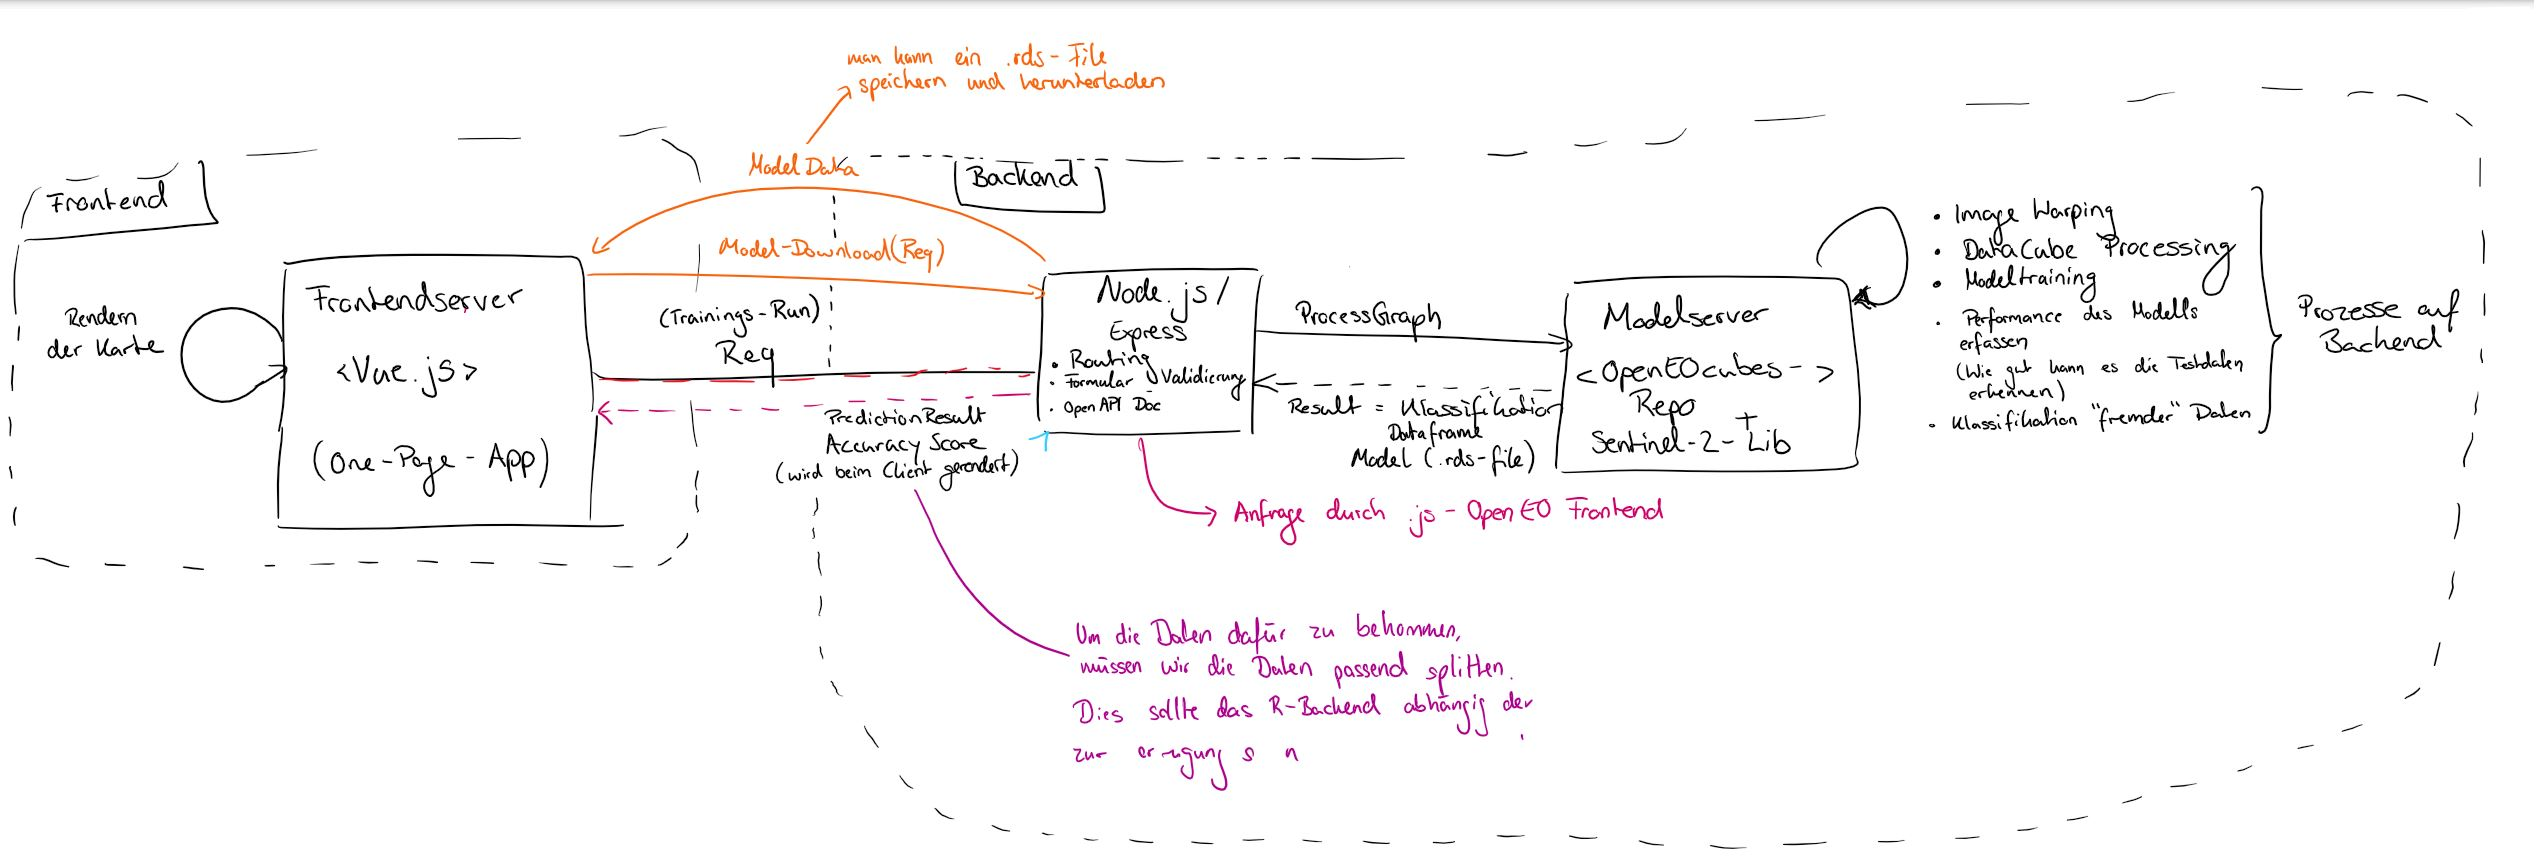
\includegraphics[scale=0.8]{Abbildungen/Serverarchitektur.JPG}
  \caption{Systemarchitektur der Applikation}
  \label{fig:systemarchitecture}
\end{figure}
\end{landscape}


\begin{landscape}
\thispagestyle{empty}
  \begin{figure}[H]
  \centering
  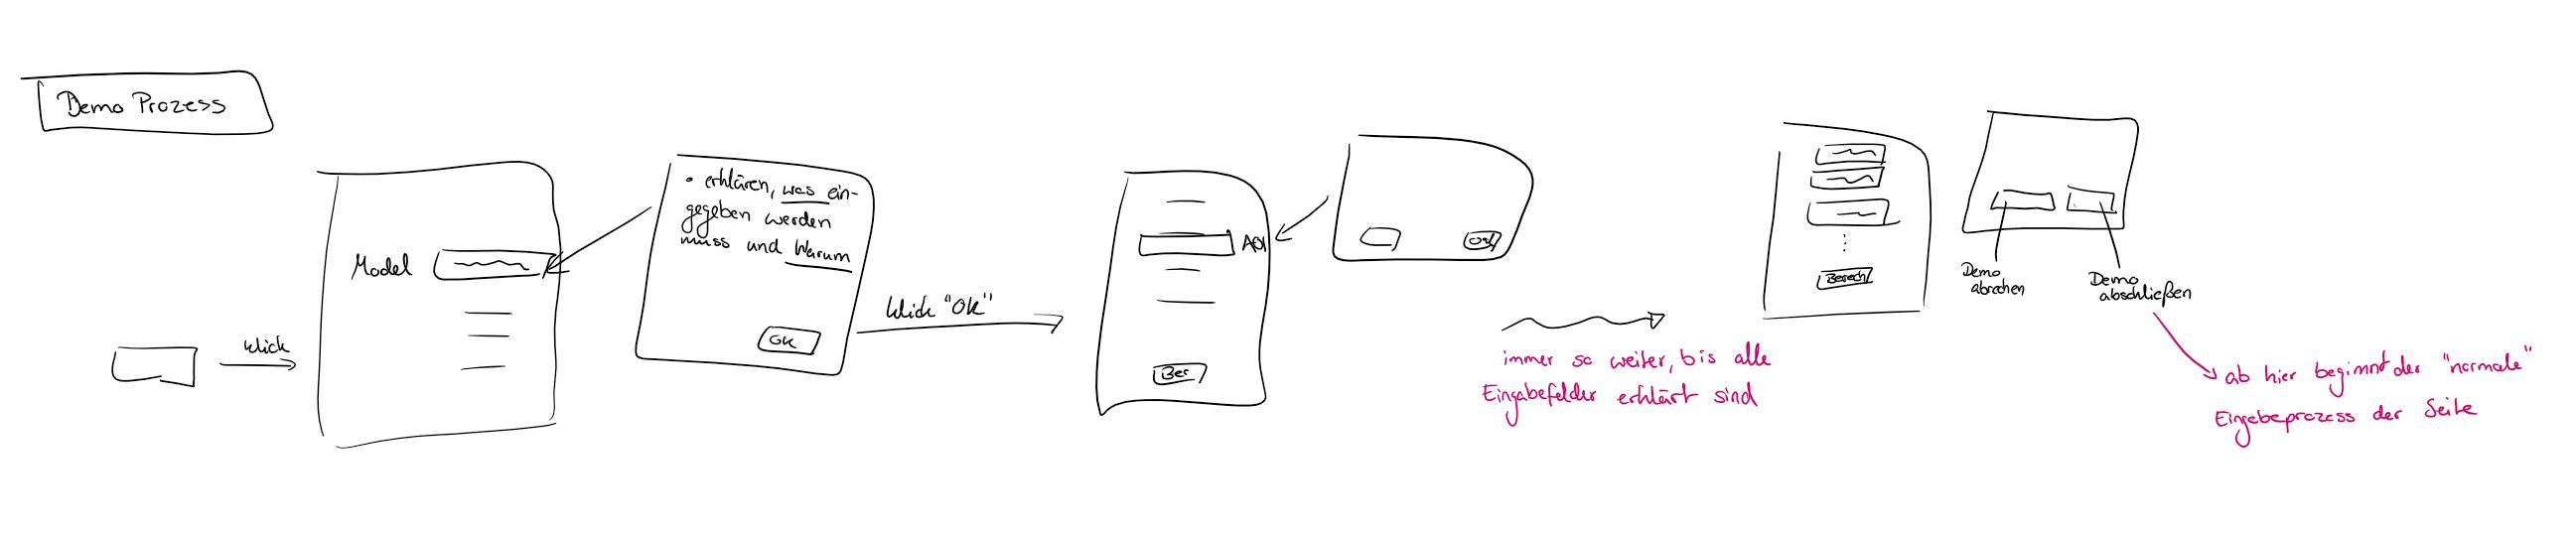
\includegraphics[scale=0.8]{Abbildungen/Demoprozess.JPG}
  \caption{Demoprozess einer Klassifikation}
  \label{fig:demoprocess}
\end{figure}
\end{landscape}

\begin{landscape}
\thispagestyle{empty}
    \begin{figure}[H]
    \centering
    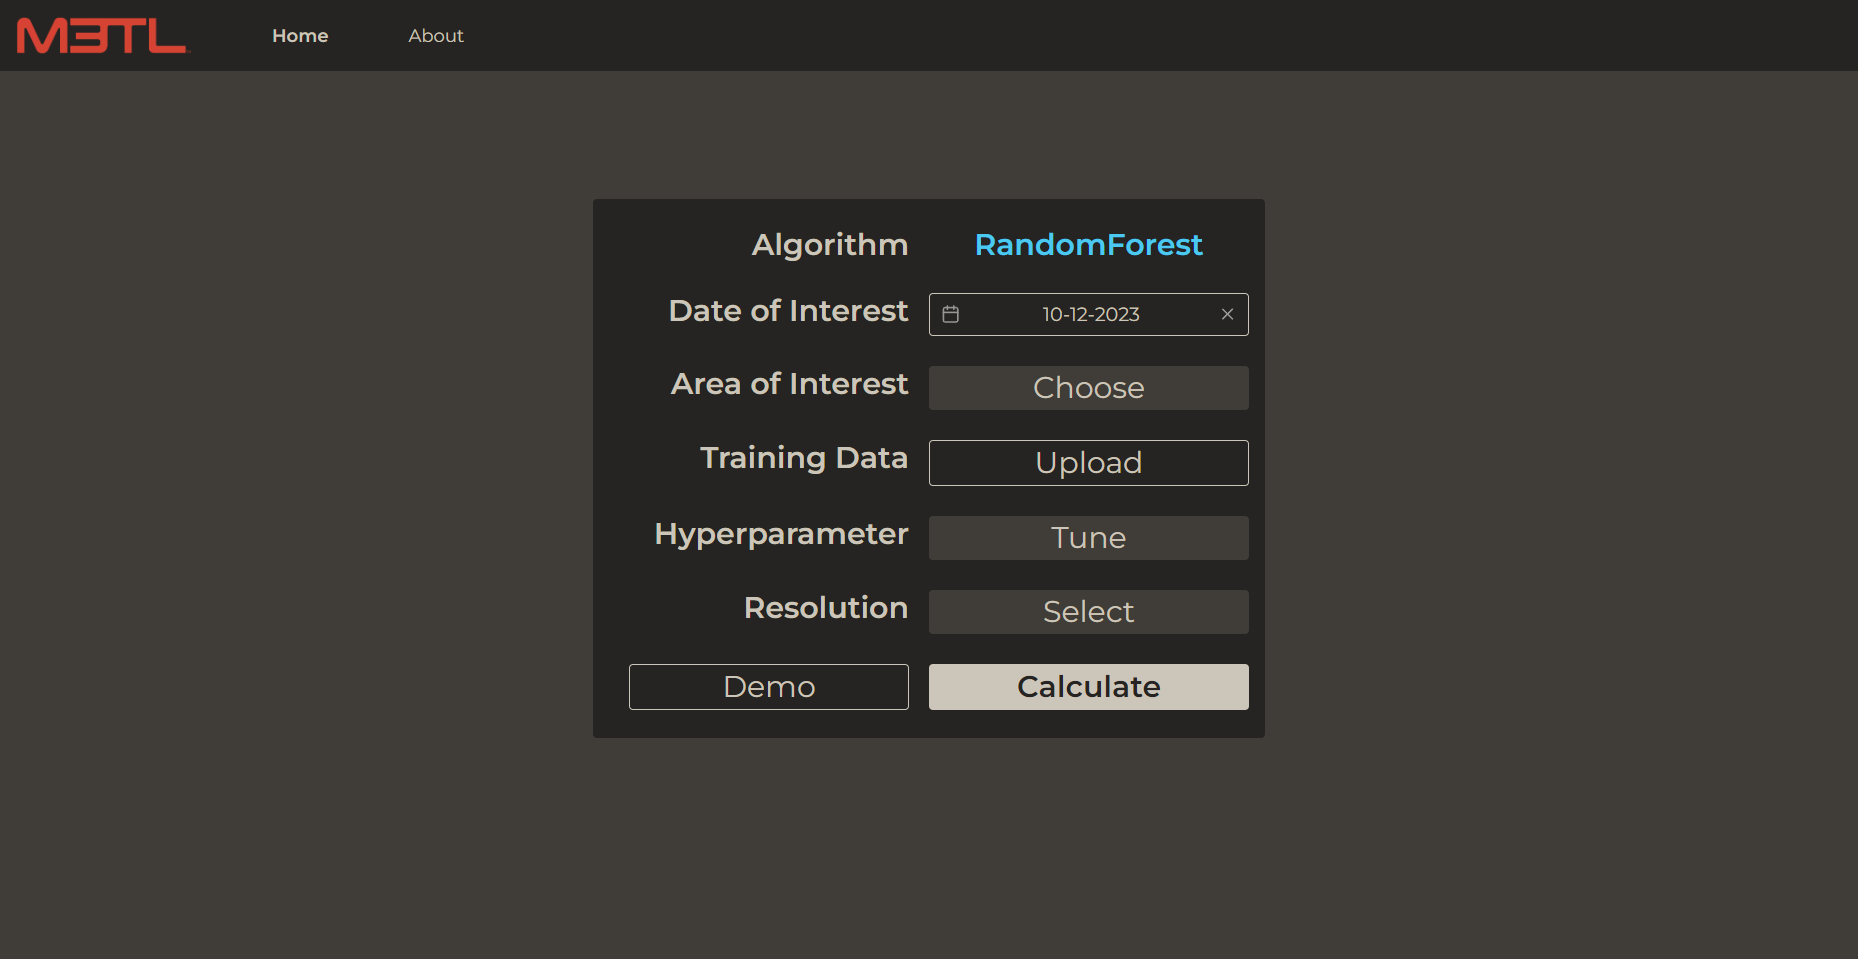
\includegraphics[scale=0.5]{Abbildungen/web-home.png}
    \caption{Die Hauptseite}
    \label{fig:homepage}
\end{figure}
\end{landscape}

\begin{figure}[H]
\centering
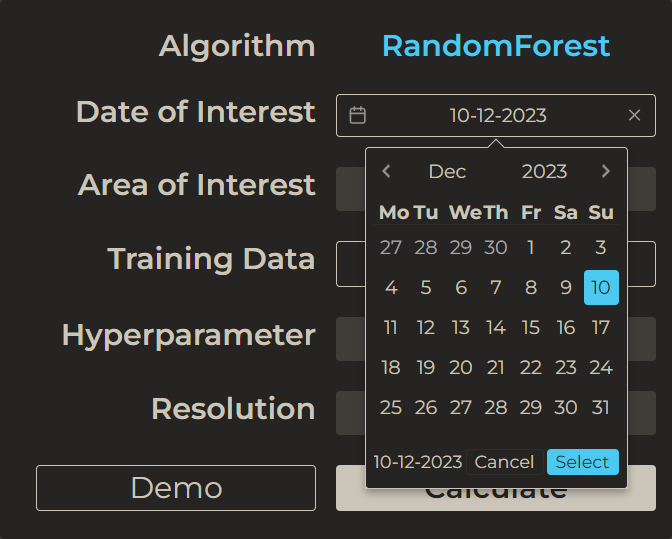
\includegraphics[scale=0.8]{Abbildungen/web-date-picker.png}
\caption{Datumsauswahl}
\label{fig:datepicker}
\end{figure}

\begin{landscape}
\thispagestyle{empty}
    \begin{figure}[H]
    \centering
    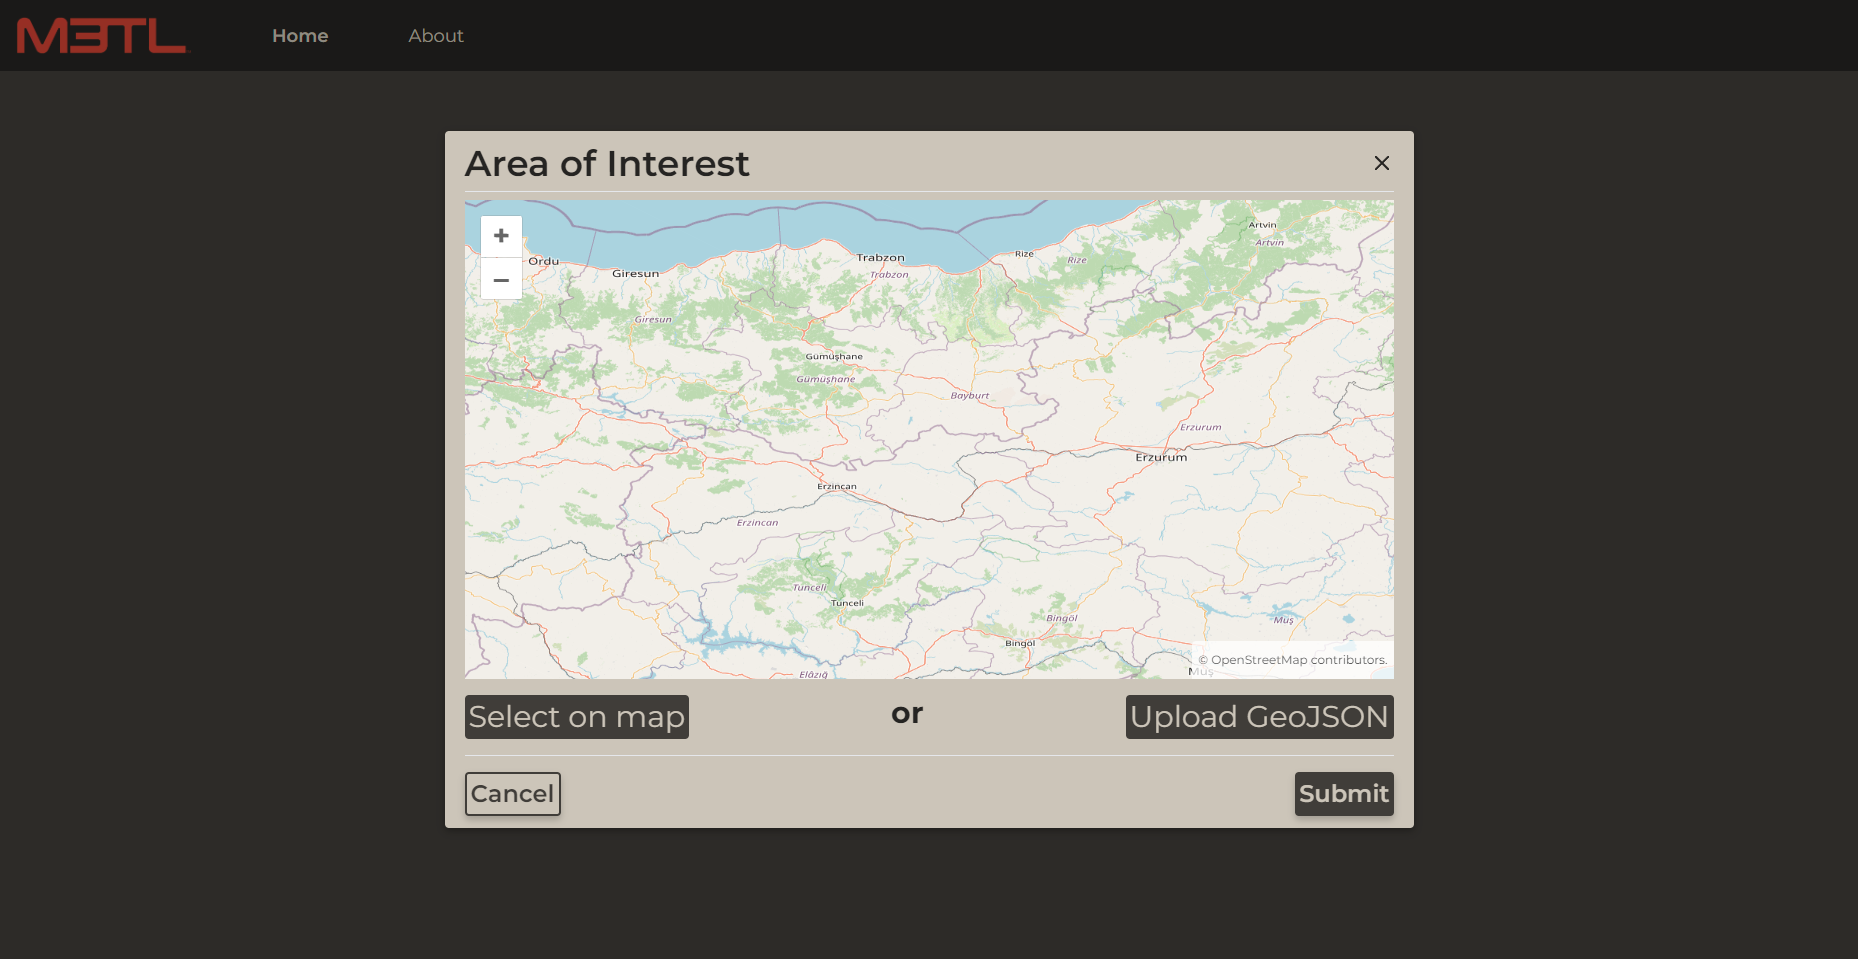
\includegraphics[scale=0.5]{Abbildungen/web-aoi.png}
    \caption{Area of Interest}
    \label{fig:aoi-modal}
\end{figure}
\end{landscape}
\end{document}
